\chapter{Einleitung}

Dieses Kapitel soll der Leser auf den Inhalt der Arbeit aufmerksam machen, ihn mit der Aufgabestellung vertraut machen und "uber die Strukturierung und Zielsetzung der Arbeit Auskunft geben.


\section{Motivation}
Objekte werden in der heutigen Tagen immer mehr mit elektronik und Inteligenz versehen. Die Leute wollen auf Grund dieser Entwicklung, dass Prozesse oder bestimmte Aufgaben ohne menschliches Eingreifen erledigt und miteinander vernetzt werden. Das System soll nur "uberwacht werden und die Ergebnisse zu bestimmte Zwecke benutz werden.

Das Internet der Dinge (in englisch \textbf{\textit{internet of things}}, Kurzform \textbf{IoT}) wird dazu benutzt, um die Interaktion zwischen Menschen und vernetzten elektronishchen Systemen zu vereinfachen.  


\section{Aufgabenstellung und Zielsetzung}
Diese Bachelorarbeit besch"aftigt sich mit der Entwicklung eines vernetzten Systems bestehend aus einem 3D Beschleunigungssesor, einem 3D Gyroskop, einem Temperatur- und Feuchtigkeitssensor. Die Sensoren messen Daten und "ubergeben diese an den STM32L475 Mikrocontroller.

Der Mikrocontroller soll die Daten verarbeiten und mit Hilfe von einem LoRa Modul drahtlos zu einem Server "ubertragen. Bevor die "ubertragung erfolgt, muss das LoRa-modul Zugang zu dem Server durch eine Gateway bekommen. Abbildung \ref{LRWAN} gibt einen gesamten "uberblick "uber den Aufbau des gesamten  Systems.

% Bild hinzufügen 
\begin{figure}[h]	
	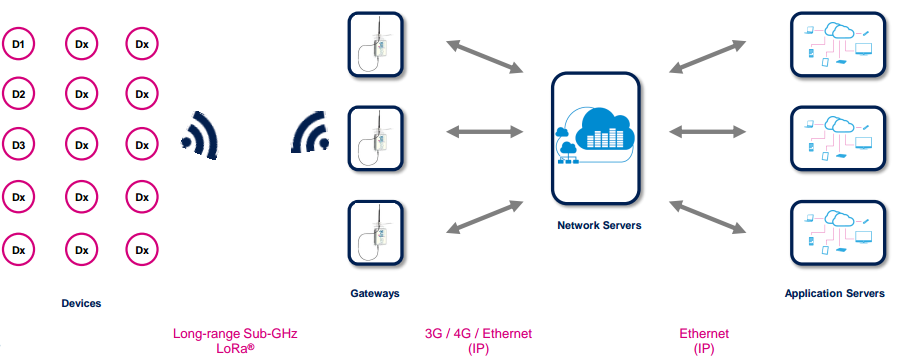
\includegraphics[width=17cm]{source/images/LoRaWAN}
	\caption{LoRaWAN Netzwerk}\label{LRWAN}
\end{figure}

\vspace{5cm}

\section{Gliederung der Arbeit}

Das Kapitel \ref{Komponente} gibt einen detaillierten "Uberblick von allen Hardware-Komponenten, die bei der Durchf"uhrung dieser Arbeit wervendet worden sind. Noch dazu kommt die Erkl"arung der Software-Entwicklung, um diese Komponenten für ein vern"unftiges Zweck anzusteuern. Als erstes wird auf die Eigenschaften von dem benutzten STM32-Nucleo Board eingegangen. Diesem Kapitel ist auch zu entnehmen, warum genau dieses Board gew"ahlt wurde. 

Als n"achstes wird das LoRa-Node und das LoRaWAN Protokol beschrieben. Dieses LoRa-Node wird dazu verwendet, um die gesammelte Daten dem Server drahtlos zu "ubertragen.

Das Kapitel \ref{G_S} erz"ahlt wie der LoRaWAN-Server und das Gateway funktionieren und zeigt die Konfugurationen, die zu "ubernehmen sind, um eine Verbindung mit einem LoRa-Node herzustellen.

Anschlei\ss{}end im Kapitel \ref{Fazit} wird eine Zusammenfassung und einen Kleinen Ausblick der Arbeit gegeben. 
   